\chapter{La reionisation} 
%réionisation et non rayonnisation!
%\section{Observation -> la reionization}
%%\section{Théorie -> La reionization}
%
%
%Qu'est ce que c'est?
%
%fin des âges sombres
%apparition des première sources de rayonnement
%Pourquoi étudier la réionisation
%
%Dernier processus impactant l'ensemble de l'univers.
%Importance pour le "missing satellite problem"
%%le manque d'observations
%%la difficulté des observations


Nous avons vu dans le chapitre precedent que lors de la recombinaison, l'Univers est passé d'un état globalement ionisé a un etat globalement neutre.
De cette transition, qui a eu lieu a enciron 380000ans après le BB, en a resulté l'emission du CMB.
Suite a cette etape, l'univers etait alors homogene, et sa dynamique etait régie essentiellement par la lutte entre l'expansion et la gravitation.
Du fait que l'univers etait neutre, le rayonnemenmt n'etait pas en mesure de se propager librement.
C'etait les ages sombres.

Il faudra alors attendre plusieurs centaine de million d'année pour voir apparaire des surdensité de gas suffisemment compactes pour former les première étoiles.
Ces premières sources lumineuses ont emmis un puissant rayonnement ionisant qui a a nouveau séparé les protons et les electron formé lors de la recombinaison.
Il a fallut encore plusieur centaine de million d'année pour que les première sources de rayonnement soient suffisement nombreuses pour que leurs photons remplissent l'univers, et le fasse passer d'un etat majoritairement neutre, a un etat a nouveau majoritairement ionisé. 
Cette transition s'appele l'epoque de la reionisation.

Une des difficultés de l'etude de la periode de reionization est que celle si a eu lieu tot dans l'histoire de l'univers lors de son premier milliard d'années.
Cette distance temporelle impose de regarder loin spatialement et donc de disposer de moyen observationnels important.
Nous somme au balbutiement des observation de la reionisation.
Dans cette section, je vais presenter quelques unes des preuvent observationnelles de la reionisation. 

\subsection{Sphère de Stromgren}

On considere une source ponctuelle dans un milieu homogene d'hydrogene neutre.
Quelle region cette source va ioniser autour d'elle?


En considerant l'équilibre entre $\dot{N_\gamma}$ le nombre de photons emis par la source et le taux de recombinaison du milieu (caractérisé par $\alpha_B(T)$ le coefficient de recombinaison en fonction de la température et $n_H$ la densité d'hydrogène neutre), \cite{stromgren_physical_1939} a exprimé l'évolution du rayon de la sphère ionizée $r_i(t)$.


\begin{equation}
\frac{dr_i(t)^3}{dt} = -n_H \alpha_B(T)r_i (t)^3 + \frac{3 \dot{N_\gamma} }{4 \pi n_H}
\end{equation}


La solution de cette équation est de la forme :

\begin{equation}
r(t) = r_s \left( 1 - e^{-t\cdot \alpha_B(T) n_H } \right)^{1/3}
\end{equation}

%
%\begin{equation}
%t_{rec} = \left( \alpha_B(T) n_H \right) ^{-1}
%\end{equation}

Le rayon de Strömgren est défini comme étant la solution stationnaire de cette équation:

\begin{equation}
r_s = \left( \frac{3 \dot{N_\gamma} }{4 \pi \alpha_B(T) n_H^2} \right)
\end{equation}



\subsection{spectre de quasar et epaisseur optique lyman alpha}
Les quasars sont des objets tres brillants qui peuvent être observé a tres grandes distance.
Les plus lointains d'entre eux presentent  un tunnel gun peterson.

Lorsqu'un photon d'une energie proche 

\begin{figure}[bth]
        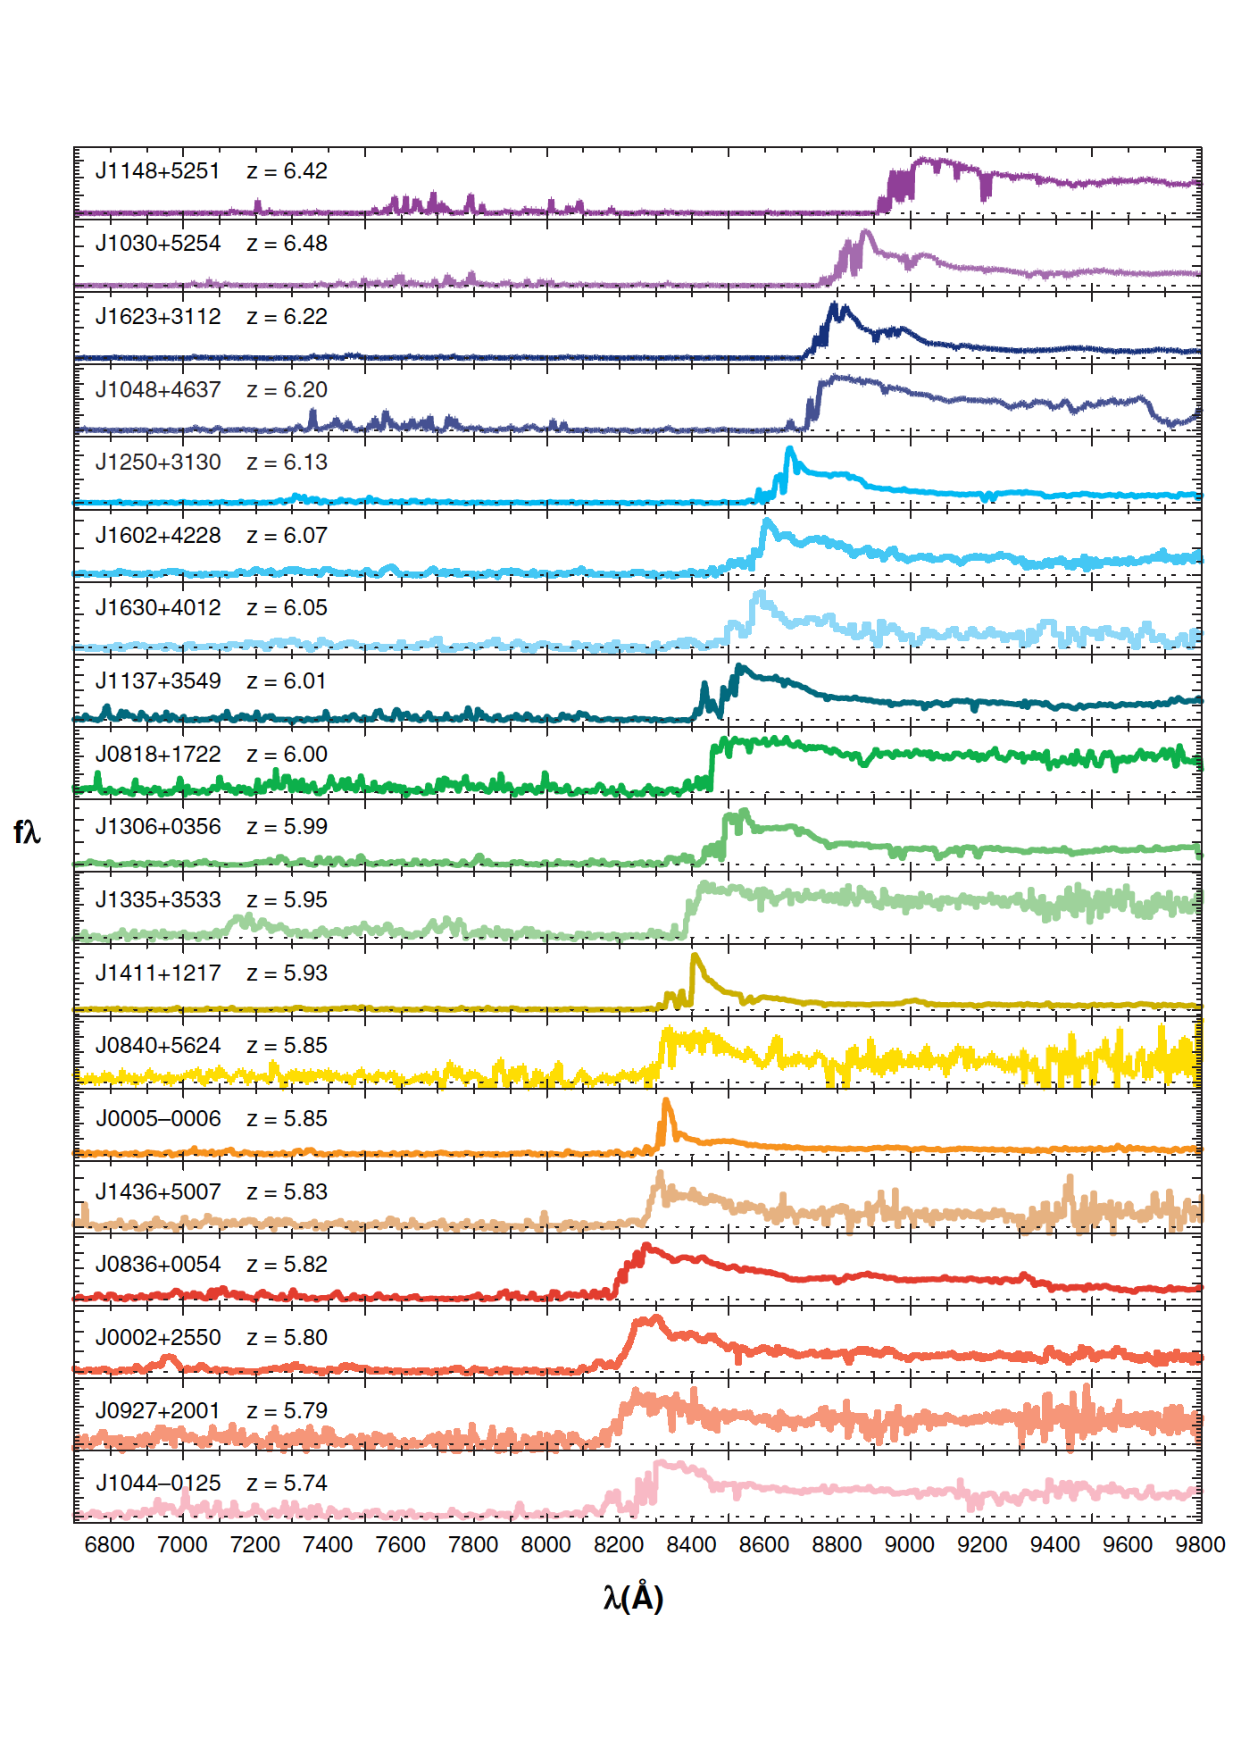
\includegraphics[width=.95\linewidth]{img/01/quasar_spectre.pdf} 
        \caption{Spectre de quasar a differents redshift presentant un tunnel gun peterson.
        Image fan et al.}
 		\label{fig:spectre_quasar}
\end{figure}


\begin{figure}[bth]
        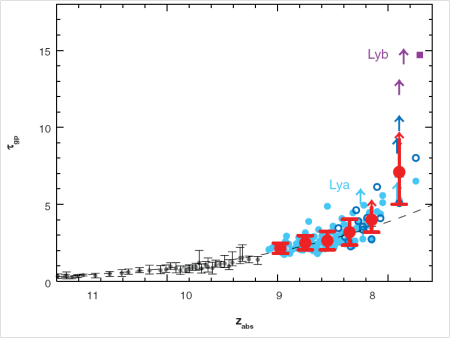
\includegraphics[width=.95\linewidth]{img/01/epaisseur_optique_quasar.png} 
        \caption{%https://ism2009.wordpress.com/2009/04/28/on-the-density-of-neutral-hydrogen-in-intergalactic-space/
		Epaisseur optique calculée a partir des spectres de quasar de la Fig\,\ref{fig:spectre_quasar}
        Image fan et al.}
 		\label{fig:epaisseur_optique_quasar}
\end{figure}

\subsection{CMB et epaisseur optique Thomson}


Les photons du CMB ont été influencé par l'avant plan constitué par la reionisation.


\begin{equation}
\tau_z = c \sigma_t \int_z^0 n_e (z) \frac{dt}{dz} dz
\end{equation}


$\sigma_t$ section efficace Thomson, $n_e (z)$ est la densité d'électron libre.


Fig \ref{fig:epaisseur_optique_thomson}


\begin{figure}[bth]
        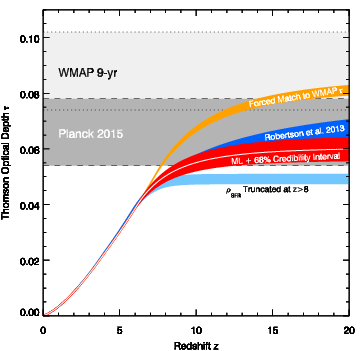
\includegraphics[width=.95\linewidth]{img/01/epaisseur_optique_thomson.png} 
        \caption{%https://inspirehep.net/record/1343310/plots
		Epaisseur optique Thomson
        Image Robertson et al.}
 		\label{fig:epaisseur_optique_thomson}
\end{figure}



\subsection{polarisation du CMB)}

\subsection{ligne 21 cm}

\subsection{fonction de luminosité UV}


\subsection{les futures observations}

Quelles sont les preuves de la réionisation?




\subsection{les principales question en suspend de l'étude de la réionisation}

%quand est ce arrivé?
%quelles sont les sources? -> débat galaxies vs quasars

La question de la provenance des photons qui ont reionizé l'univers est toujours en suspend.
En utilisisant la halo mass function presenté en TODO REF, on observe que les galaxies les moins massives sont nombreuse et que les galaxies les plus massives sont rare.
Or, plus une galaxie est massive, plus celle ci va créer des étoiles, et donc emmetres des photons.
La balance entre les nombreuses galaxies peu lumineuses, et les rare galaxies extremenet lumineuse reste a determiner

De plus, les quasars, objet extremement lumineux, situé dans les galaxies les plus massives, augmente encore le budget de photon.
L'inconnue est que pour creer un quasar, une grande quantité de matière est necessaire.
Il reste a établir si au redshift considéré
\cite{chardin_large-scale_2017}


La figure \ref{fig:gal_AGN} extraite de \cite{trac_computer_2011} presente le budget de photon plausible pour les galaxies ou les quasars.
Dans le cadre de cette thèse, les sources considérées sont exclusivement les galaxies.

\begin{figure}[bth]
        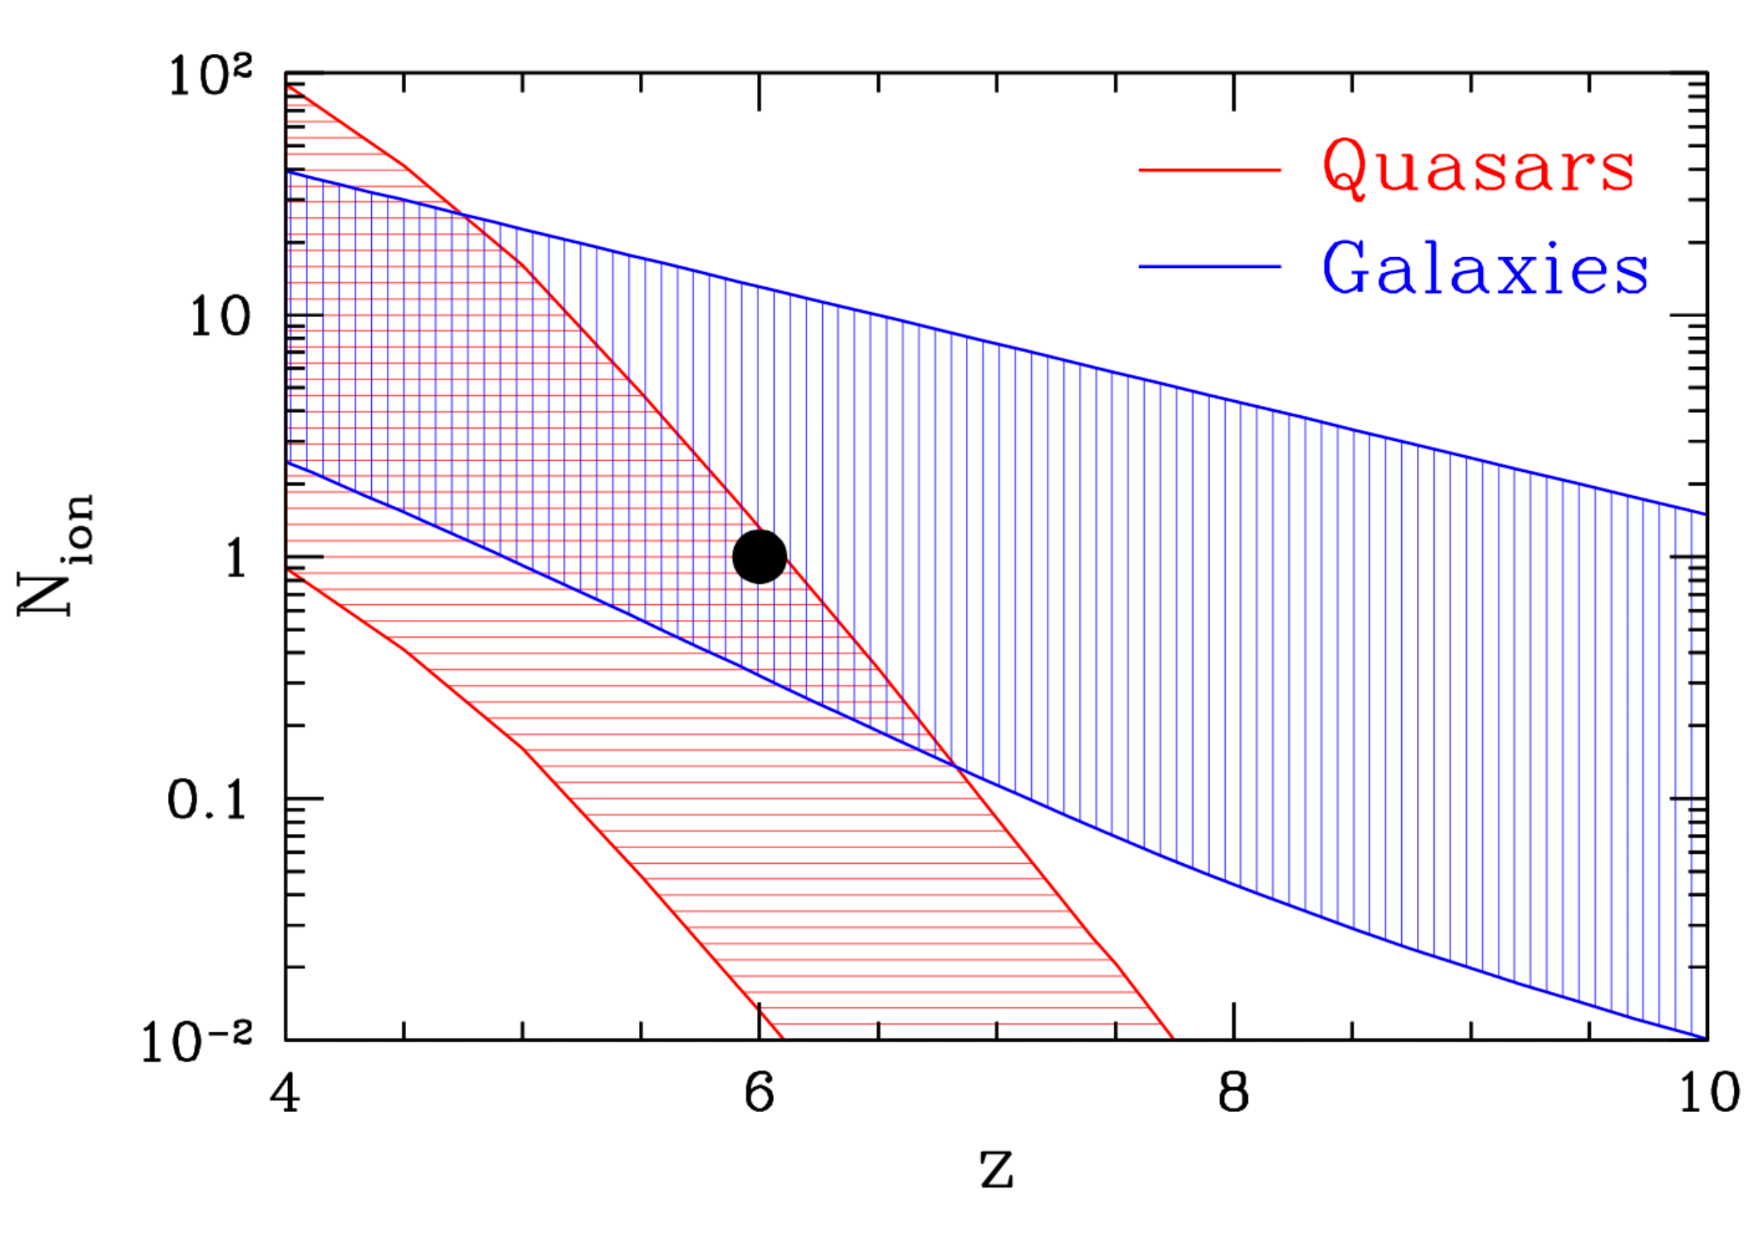
\includegraphics[width=.95\linewidth]{img/01/gal_AGN.pdf} 
        \caption{
        Budget de photons provenant des galaxies et des quasars qurant la reionization.
}
 		\label{fig:gal_AGN}
\end{figure}

outlier dans l'épaisseur optique des quasars
Le groupe local ?
